\chapter{Opérateurs, observables et matrices de Pauli}

Une bonne notation n’est pas un simple ornement. Dans une discipline fondée sur des vecteurs abstraits et des nombres complexes, une notation qui permet de manipuler les symboles sans devoir sans cesse les traduire en mots fait partie intégrante de l’outillage. La notation bra--ket de Dirac est précieuse précisément pour cette raison : elle rend visible la géométrie de l’espace des états tout en permettant de calculer avec des composantes et des matrices.

Notre tâche immédiate est mathématique. Nous allons introduire les opérateurs linéaires, apprendre comment ils agissent aussi bien sur les bras que sur les kets, puis isoler la classe particulière des opérateurs hermitiens. Ce n’est qu’ensuite que nous leur associerons les notions physiques d’\emph{observable}, de \emph{résultat de mesure} et de \emph{probabilité}. Nous verrons ainsi apparaître les trois observables de spin sous la forme des matrices de Pauli, au lieu de nous les voir présenter comme des objets à mémoriser.

\section{Bases orthonormées et composantes}

Les états forment un espace vectoriel complexe. On peut additionner ses vecteurs ket et les multiplier par des nombres complexes. À chaque ket \(\ket{A}\) est associé un bra \(\bra{A}\), obtenu par l’opération de conjugaison-dualité. Une base n’est pas unique, mais, une fois choisie, elle permet de décrire chaque vecteur par ses composantes dans cette base.

Soit
\[
\bigl\{\ket{1},\ket{2},\ldots,\ket{N}\bigr\}
\]
une base orthonormée. L’orthogonalité et la normalisation s’expriment par
\begin{equation}
\braket{j}{i}=\delta_{ji}.
\label{eq:orthonormal-basis}
\end{equation}
Ici, \(\delta_{ji}\) vaut un lorsque \(j=i\) et zéro dans le cas contraire. La dimension \(N\) est le nombre maximal de directions mutuellement orthogonales dans l’espace ; une base orthonormée complète contient exactement autant de vecteurs.

Développons un ket quelconque :
\begin{equation}
\ket{A}=\sum_i \alpha_i\ket{i}.
\label{eq:ket-expansion}
\end{equation}
Les coefficients n’ont rien de mystérieux. Multiplions à gauche par \(\bra{j}\) :
\begin{align}
\braket{j}{A}
 &=\sum_i\alpha_i\braket{j}{i} \\
 &=\sum_i\alpha_i\delta_{ji}
 =\alpha_j.
\end{align}
On obtient donc
\begin{equation}
\alpha_i=\braket{i}{A}.
\label{eq:components-inner-products}
\end{equation}
La composante d’indice \(i\) est la projection de \(\ket{A}\) sur la direction de base d’indice \(i\).

En reportant l’équation~\eqref{eq:components-inner-products} dans l’équation~\eqref{eq:ket-expansion}, on obtient une forme particulièrement utile :
\begin{equation}
\ket{A}=\sum_i\ket{i}\braket{i}{A}.
\label{eq:ket-completeness-action}
\end{equation}
Cette somme n’a rien changé au vecteur ; elle l’a simplement décomposé selon les directions de la base, puis recomposé. Nous aurons souvent recours à cette opération. On la décrit généralement comme \emph{l’insertion d’un ensemble complet d’états}, car
\begin{equation}
\sum_i\ket{i}\bra{i}=\mathbf 1.
\label{eq:resolution-identity}
\end{equation}

Le développement correspondant pour un bra est
\begin{equation}
\bra{A}=\sum_i\braket{A}{i}\bra{i}
       =\sum_i\alpha_i^*\bra{i}.
\label{eq:bra-expansion}
\end{equation}
La conjugaison complexe de \(\alpha_i\) est essentielle. Transformer un ket en bra conjugue chacun de ses coefficients numériques.

\begin{figure}[htbp]\centering
\includegraphics[width=0.82\textwidth]{lecture_03_figure_04.png}\caption{Les deux règles qui définissent un opérateur linéaire, présentées après le rappel sur les bases.}\lectureframe{00:12:44}\end{figure}

\section{Les opérateurs linéaires comme machines}

Un opérateur linéaire \(M\) est une règle qui associe à un ket d’entrée un ket de sortie unique. Une image utile, due à John Wheeler, est celle d’une machine dotée d’un port d’entrée et d’un port de sortie : on introduit \(\ket{A}\), on actionne la machine et l’on obtient \(M\ket{A}\). L’entrée détermine la sortie. La réciproque n’est pas nécessairement unique : deux entrées peuvent donner la même sortie, et il se peut qu’aucune machine inverse n’existe.

L’adjectif \emph{linéaire} recouvre deux règles. Pour un nombre complexe \(z\),
\begin{align}
M\bigl(z\ket{A}\bigr)&=z\,M\ket{A}, \label{eq:operator-homogeneous}\\
M\bigl(\ket{A}+\ket{B}\bigr)&=M\ket{A}+M\ket{B}.
\label{eq:operator-additive}
\end{align}
Un scalaire traverse la machine sans changement, et une somme peut être traitée terme à terme. Ces règles impliquent également la linéarité pour toute combinaison linéaire complexe finie.

La même idée s’applique aux vecteurs ordinaires de l’espace à trois dimensions. La mécanique quantique n’invente pas les applications linéaires. Elle les rend indispensables parce que l’espace des états est abstrait et complexe, et parce que les grandeurs mesurables seront représentées par une famille particulière de telles applications.

\section{D’un opérateur à sa matrice}

Supposons que la machine transforme \(\ket{A}\) en \(\ket{B}\) :
\begin{equation}
M\ket{A}=\ket{B}.
\label{eq:operator-action}
\end{equation}
Choisissons la même base orthonormée pour l’entrée et la sortie, et écrivons
\[
\ket{A}=\sum_j\alpha_j\ket{j},
\qquad
\ket{B}=\sum_i\beta_i\ket{i}.
\]
Pour trouver la composante de sortie d’indice \(i\), projetons l’équation~\eqref{eq:operator-action} à l’aide de \(\bra{i}\) :
\begin{equation}
\bra{i}M\ket{A}=\braket{i}{B}=\beta_i.
\end{equation}
Introduisons maintenant le développement de \(\ket{A}\) :
\begin{align}
\bra{i}M\ket{A}
 &=\sum_j\bra{i}M\ket{j}\braket{j}{A}\\
 &=\sum_j\bra{i}M\ket{j}\alpha_j
 =\beta_i.
\end{align}
Les nombres
\begin{equation}
m_{ij}\equiv\bra{i}M\ket{j}
\label{eq:matrix-elements}
\end{equation}
sont les \emph{éléments de matrice} de \(M\) dans la base choisie. Par conséquent,
\begin{equation}
\boxed{\sum_jm_{ij}\alpha_j=\beta_i.}
\label{eq:component-action}
\end{equation}

\begin{figure}[htbp]\centering
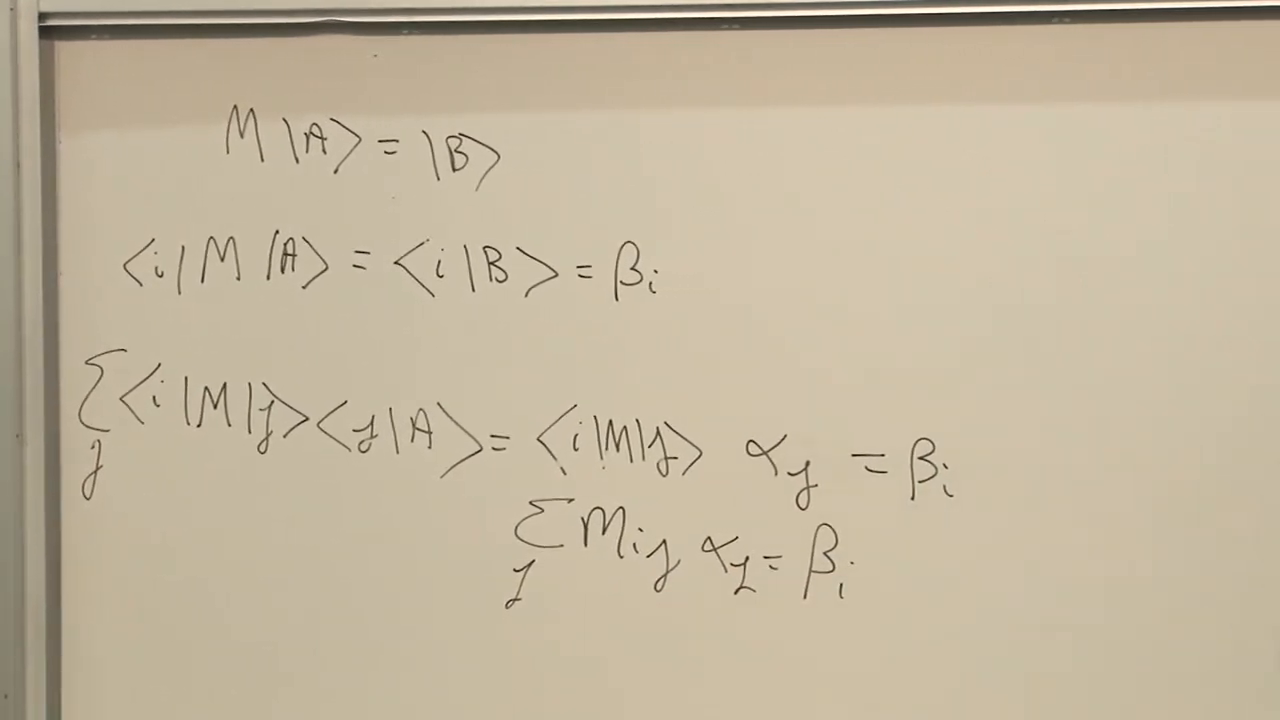
\includegraphics[width=0.84\textwidth]{lecture_03_figure_02.png}\caption{L’équation abstraite \(M\ket{A}=\ket{B}\), projetée et décomposée en la règle sur les composantes \(\sum_jm_{ij}\alpha_j=\beta_i\).}\lectureframe{00:18:30}\end{figure}

Si l’espace est de dimension \(N\), les \(N^2\) nombres \(m_{ij}\) forment une matrice carrée \(N\times N\). L’équation~\eqref{eq:component-action} s’écrit exactement
\begin{equation}
\begin{pmatrix}
m_{11}&m_{12}&\cdots&m_{1N}\\
m_{21}&m_{22}&\cdots&m_{2N}\\
\vdots&\vdots&\ddots&\vdots\\
m_{N1}&m_{N2}&\cdots&m_{NN}
\end{pmatrix}
\begin{pmatrix}
\alpha_1\\
\alpha_2\\
\vdots\\
\alpha_N
\end{pmatrix}
=
\begin{pmatrix}
\beta_1\\
\beta_2\\
\vdots\\
\beta_N
\end{pmatrix}.
\label{eq:matrix-vector-action}
\end{equation}
Pour obtenir \(\beta_1\), multiplions la première ligne par la colonne d’entrée et faisons la somme ; répétons l’opération avec la deuxième ligne pour obtenir \(\beta_2\), et ainsi de suite. La matrice est la réalisation concrète de la machine de Wheeler.

\begin{figure}[htbp]\centering
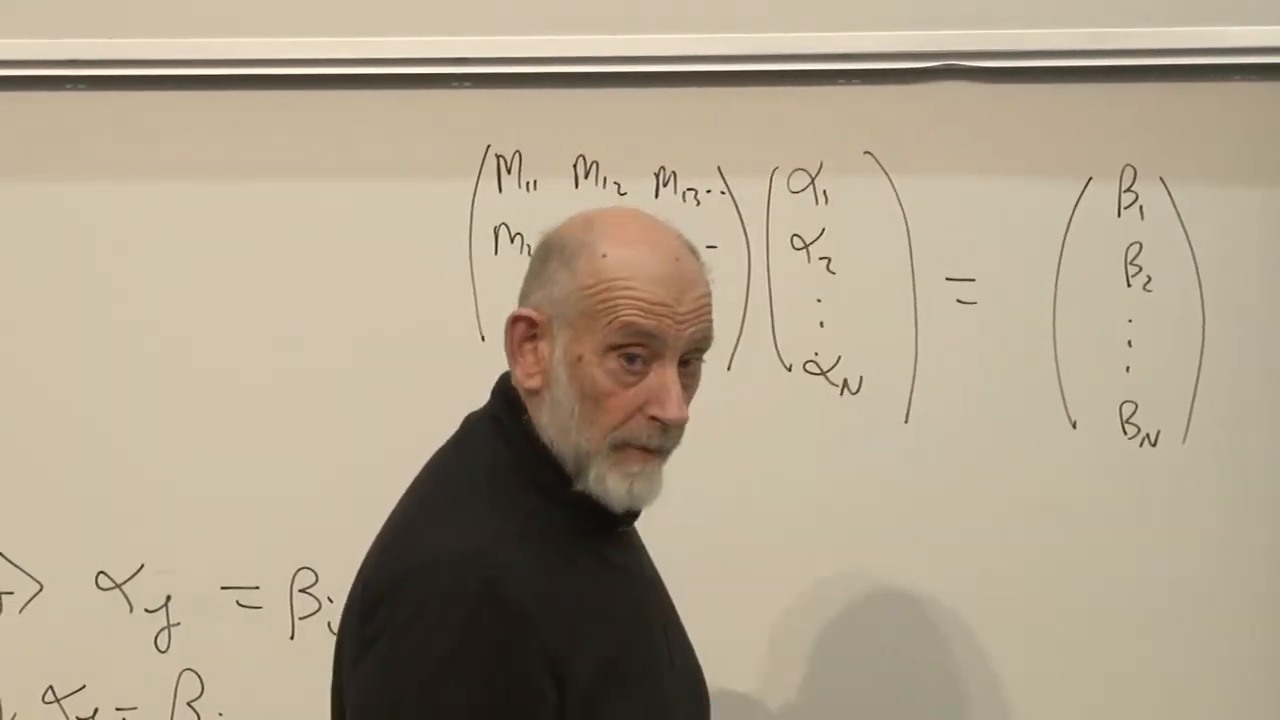
\includegraphics[width=0.84\textwidth]{lecture_03_figure_03.png}\caption{L’action du même opérateur, représentée par une matrice carrée multipliant la colonne des coefficients d’entrée.}\lectureframe{00:20:01}\end{figure}

Nous avons obtenu un algorithme, mais perdu une partie de la géométrie qui était visible. L’énoncé abstrait \(M\ket{A}=\ket{B}\) ne dépend pas des coordonnées. Les éléments particuliers \(m_{ij}\), \(\alpha_j\) et \(\beta_i\) dépendent, eux, de la base choisie. Une autre base orthonormée modifie ces trois tableaux, tout en laissant inchangés l’application sous-jacente et ses prédictions physiques.

\begin{classroomqa}\audiencequestion{Le choix de la base peut-il déterminer si un problème est soluble ?}\lecturerresponse{Il peut déterminer si la solution est facile à voir. Une base bien choisie peut rendre un opérateur diagonal et le calcul presque immédiat ; une base mal choisie peut dissimuler la structure sous une algèbre pénible. Elle ne peut pas modifier le résultat d’une expérience. Si deux bases conduisent à des résultats physiques différents, le calcul est faux.}\end{classroomqa}

\section{Bras, kets et antilinéarité}

\begin{classroomqa}\audiencequestion{Un opérateur linéaire peut-il transformer un ket en bra, ou un bra en ket ?}\lecturerresponse{Pas un opérateur linéaire ordinaire tel que nous venons de le définir. Celui-ci associe des kets à des kets, et les scalaires complexes passent sans changement. L’opération qui échange les kets et les bras conjugue aussi leurs coefficients ; elle appartient donc à une autre classe.}\end{classroomqa}

La multiplication par un nombre complexe fixé est un opérateur linéaire simple. La conjugaison complexe ne l’est pas. Si \(K\) désigne la conjugaison, alors
\[
K\bigl(z\ket{A}\bigr)=z^*K\ket{A},
\]
et non \(zK\ket{A}\). Une telle application est dite \emph{antilinéaire}. Ce terme ne signifie pas qu’elle est le contraire de la linéarité ; il indique que les scalaires sont conjugués. Son lien plus profond avec les antiparticules dépasse le cadre de cette discussion.

Les opérateurs linéaires peuvent néanmoins agir sur les bras. Par convention, on écrit l’opérateur à droite :
\begin{equation}
\bra{A}M.
\end{equation}
Cette définition est choisie de façon à ce qu’un élément de matrice ne prête pas à confusion au niveau des crochets :
\begin{equation}
\bra{A}\bigl(M\ket{B}\bigr)
=
\bigl(\bra{A}M\bigr)\ket{B}
\equiv
\bra{A}M\ket{B}.
\label{eq:bracket-independence}
\end{equation}

Pour comprendre pourquoi cela est possible, développons les deux vecteurs :
\begin{align}
\bra{A}M\ket{B}
 &=\left(\sum_i\alpha_i^*\bra{i}\right)
   M
   \left(\sum_j\beta_j\ket{j}\right)\\
 &=\sum_{ij}\alpha_i^*m_{ij}\beta_j.
\label{eq:matrix-element-double-sum}
\end{align}
C’est une somme double ordinaire. On peut d’abord sommer sur \(j\) et considérer que \(M\) agit sur le ket, ou sommer d’abord sur \(i\) et considérer qu’il agit sur le bra. Le résultat est le même. Cette notation a précisément été conçue pour éviter les crochets superflus.

\section{L’opération dagué}

Il existe une seconde question, différente, concernant l’action du côté des bras. Supposons que
\[
M\ket{A}=\ket{B}.
\]
Quel opérateur transforme le bra correspondant \(\bra{A}\) en \(\bra{B}\) ? En général, ce n’est pas \(M\) lui-même. Si \(M\) correspondait à la multiplication par un nombre complexe \(z\), l’équation pour le ket serait \(\ket{B}=z\ket{A}\), tandis que celle pour le bra serait \(\bra{B}=z^*\bra{A}\).

L’opérateur recherché se note \(M^\dagger\) ; c’est le \emph{conjugué hermitien} de \(M\), défini par
\begin{equation}
M\ket{A}=\ket{B}
\quad\Longleftrightarrow\quad
\bra{A}M^\dagger=\bra{B}.
\label{eq:dagger-definition}
\end{equation}
Le dagué est l’analogue, pour les opérateurs, de la conjugaison complexe.

La règle matricielle s’en déduit directement. Soit
\[
M\ket{i}=\ket{i'}.
\]
Alors
\[
m_{ji}=\bra{j}M\ket{i}=\braket{j}{i'}.
\]
La relation daguée pour le bra est \(\bra{i}M^\dagger=\bra{i'}\), d’où
\[
(m^\dagger)_{ij}
=\bra{i}M^\dagger\ket{j}
=\braket{i'}{j}.
\]
Inverser un produit scalaire le conjugue :
\[
\braket{i'}{j}=\braket{j}{i'}^*.
\]
Par conséquent,
\begin{equation}
\boxed{(m^\dagger)_{ij}=m_{ji}^*.}
\label{eq:dagger-matrix-elements}
\end{equation}

\begin{figure}[htbp]\centering
\includegraphics[width=0.84\textwidth]{lecture_03_figure_05.png}\caption{La relation complète au tableau pour la conjugaison hermitienne : on échange les indices et on prend le conjugué complexe.}\lectureframe{00:42:23}\end{figure}

En notation matricielle, on transpose puis on conjugue :
\begin{equation}
\begin{pmatrix}
a&b\\
c&d
\end{pmatrix}^{\!\dagger}
=
\begin{pmatrix}
a^*&c^*\\
b^*&d^*
\end{pmatrix}.
\label{eq:dagger-two-by-two}
\end{equation}
La transposition réfléchit les éléments par rapport à la diagonale principale ; la conjugaison remplace chaque \(i\) par \(-i\). Par exemple,
\begin{equation}
\begin{pmatrix}
2&6+7i\\
4-i&9+i
\end{pmatrix}^{\!\dagger}
=
\begin{pmatrix}
2&4+i\\
6-7i&9-i
\end{pmatrix}.
\label{eq:dagger-numerical-example}
\end{equation}
Les éléments diagonaux restent à leur place, mais sont conjugués, tandis que les deux éléments hors diagonale échangent leur position et sont conjugués.

\section{Opérateurs hermitiens}

Un nombre complexe est réel si et seulement s’il est égal à son conjugué complexe. L’analogue pour les opérateurs s’énonce immédiatement.

\begin{definition}Un opérateur \(M\) est \emph{hermitien} lorsque
\begin{equation}
M=M^\dagger.
\label{eq:hermitian-definition}
\end{equation}
De manière équivalente, dans toute base orthonormée,
\begin{equation}
m_{ij}=m_{ji}^*.
\label{eq:hermitian-components}
\end{equation}\end{definition}

Posons \(i=j\) dans l’équation~\eqref{eq:hermitian-components}. Alors
\[
m_{ii}=m_{ii}^*,
\]
Tous les éléments diagonaux sont donc réels. Hors de la diagonale, les éléments apparaissent par paires conjuguées et symétriques par réflexion. Si l’un des éléments vaut \(4-i\), son symétrique vaut \(4+i\) ; si l’un vaut le nombre réel \(5\), son symétrique aussi.

\begin{figure}[htbp]\centering
\includegraphics[width=0.78\textwidth]{lecture_03_figure_06.png}\caption{Exemple complet de matrice hermitienne : éléments réels sur la diagonale et paires de conjugués complexes symétriques par réflexion par rapport à celle-ci.}\lectureframe{00:45:43}\end{figure}

Les opérateurs hermitiens sont importants parce qu’ils représenteront les grandeurs mesurables. Avant d’établir cette correspondance, nous devons comprendre leurs directions propres.

\section{Vecteurs propres et directions propres}

Lorsqu’on découvre les vecteurs propres, cette partie peut sembler aller plus vite que la physique qui l’entoure. Il s’agit d’algèbre linéaire standard, et non d’une nouvelle hypothèse physique ; si ces notions ne vous sont pas familières, prenez le temps de revoir tranquillement les définitions, puis revenez à l’argument.

Un opérateur général modifie la direction d’un vecteur. Par exemple, une rotation dans l’espace ordinaire à trois dimensions détourne presque tous les vecteurs de leur direction initiale. L’axe de rotation fait exception : un vecteur porté par cet axe conserve sa direction. C’est le modèle d’un vecteur propre.

Une rotation non triviale d’un plan réel à deux dimensions illustre la possibilité contraire : aucune direction réelle n’y reste fixe à un facteur réel près. Ainsi, un opérateur générique sur un espace réel donné n’a pas nécessairement de vecteur propre réel. Les opérateurs hermitiens des espaces complexes utilisés en mécanique quantique possèdent des propriétés beaucoup plus fortes.

Un vecteur propre de \(M\) satisfait à
\begin{equation}
M\ket{i}=\lambda_i\ket{i}.
\label{eq:eigenvalue-equation}
\end{equation}
Le nombre \(\lambda_i\) est sa valeur propre. Le vecteur propre est associé à l’opérateur ; on ne parle pas d’un vecteur propre sans préciser l’application dont il conserve la direction.

L’équation~\eqref{eq:eigenvalue-equation} ne fixe ni sa norme ni sa phase. Pour tout nombre complexe non nul \(z\),
\[
M\bigl(z\ket{i}\bigr)
=zM\ket{i}
=\lambda_i\bigl(z\ket{i}\bigr).
\]
Il est donc plus exact de parler d’une \emph{direction propre} : tout multiple non nul de \(\ket{i}\) décrit la même direction et possède la même valeur propre. Nous choisissons généralement un représentant normalisé.

Voici le fait spectral essentiel : un opérateur hermitien sur un espace vectoriel complexe de dimension \(N\) admet une base orthonormée complète de vecteurs propres, au nombre de \(N\). On peut comprendre deux aspects de cet énoncé avec très peu d’algèbre.

\subsection{Les valeurs propres hermitiennes sont réelles}

Supposons que \(M=M^\dagger\) et que
\[
M\ket{i}=\lambda_i\ket{i}.
\]
Prenons le conjugué hermitien de l’équation entière :
\begin{equation}
\bra{i}M^\dagger=\lambda_i^*\bra{i}.
\label{eq:eigen-bra-equation}
\end{equation}
Puisque \(M^\dagger=M\), multiplions l’équation pour le ket par \(\bra{i}\) et celle pour le bra par \(\ket{i}\) :
\begin{align}
\bra{i}M\ket{i}&=\lambda_i\braket{i}{i},\\
\bra{i}M\ket{i}&=\lambda_i^*\braket{i}{i}.
\end{align}
La même norme non nulle multiplie les deux nombres, donc
\begin{equation}
\lambda_i=\lambda_i^*.
\end{equation}
Toutes les valeurs propres d’un opérateur hermitien sont réelles. C’est un premier indice qu’un tel opérateur peut représenter le nombre réel affiché par un appareil de mesure.

\subsection{Des valeurs propres différentes donnent des vecteurs propres orthogonaux}

Soit
\[
M\ket{i}=\lambda_i\ket{i},
\qquad
M\ket{j}=\lambda_j\ket{j},
\]
où \(M\) est hermitien. Prenons le conjugué hermitien de la deuxième équation. On sait déjà que sa valeur propre est réelle :
\[
\bra{j}M=\lambda_j\bra{j}.
\]
Multiplions maintenant la première équation par \(\bra{j}\) et l’équation pour le bra par \(\ket{i}\) :
\begin{align}
\bra{j}M\ket{i}&=\lambda_i\braket{j}{i},\\
\bra{j}M\ket{i}&=\lambda_j\braket{j}{i}.
\end{align}
En soustrayant, on obtient
\begin{equation}
\boxed{(\lambda_i-\lambda_j)\braket{j}{i}=0.}
\label{eq:hermitian-orthogonality}
\end{equation}
Si \(\lambda_i\ne\lambda_j\), alors
\[
\braket{j}{i}=0.
\]
Les directions propres sont orthogonales.

\begin{figure}[htbp]\centering
\includegraphics[width=0.82\textwidth]{lecture_03_figure_07.png}\caption{L’étape décisive de la preuve d’orthogonalité : des valeurs propres différentes imposent l’annulation du produit scalaire.}\lectureframe{00:59:00}\end{figure}

Lorsque deux valeurs propres sont égales, l’équation~\eqref{eq:hermitian-orthogonality} n’impose aucune condition dans le sous-espace propre dégénéré. On peut y choisir une base orthonormée. Avec les autres directions propres, ces vecteurs forment la base propre orthonormée complète annoncée par le théorème spectral.

L’orthogonalité a aussi une interprétation physique. Deux états orthogonaux peuvent être distingués sans ambiguïté par une mesure appropriée. Des états propres associés à des valeurs propres différentes doivent être distinguables, puisque l’appareil indique pour eux des nombres réels différents. L’algèbre et l’interprétation opérationnelle pointent déjà vers la même correspondance.

\section{Les postulats de la mesure}

Nous disposons maintenant d’assez de formalisme pour énoncer les correspondances fondamentales de la mécanique quantique. Elles peuvent sembler étrangères au premier abord. Leur sens ne devient concret qu’à l’usage ; énonçons-les donc clairement, puis revenons aussitôt à l’expérience de spin.

Une mesure unique produit un nombre réel. On peut regrouper deux résultats réels compatibles dans un nombre complexe, mais ce regroupement contient toujours deux mesures. Le résultat élémentaire d’un détecteur est réel. Les opérateurs hermitiens sont donc les candidats naturels : leurs valeurs propres sont réelles et leurs vecteurs propres forment une base orthonormée complète.

\begin{enumerate}\item Une grandeur mesurable, ou \emph{observable}, est représentée par un opérateur hermitien \(M\).
\item Les résultats possibles de la mesure de \(M\) sont ses valeurs propres \(\lambda_i\).
\item Un état dans lequel \(M\) a la valeur déterminée \(\lambda_i\) est un état propre \(\ket{i}\) qui satisfait à
\[
M\ket{i}=\lambda_i\ket{i}.
\]
\item Si le système est dans un état général normalisé \(\ket{A}\), la probabilité d’obtenir \(\lambda_i\) vaut
\begin{equation}
P(\lambda_i\mid A)
=\left|\braket{i}{A}\right|^2
=\braket{i}{A}\braket{A}{i}.
\label{eq:born-rule}
\end{equation}\end{enumerate}

Cette liste constitue un point de départ commode, mais ne forme pas nécessairement un système minimal d’axiomes indépendants ; dans une formulation plus économique, certains énoncés peuvent se déduire des autres. Présenter séparément ces correspondances permet de mieux distinguer leurs rôles physiques.

Le nombre complexe \(\braket{i}{A}\) est une \emph{amplitude de probabilité}, et non une probabilité. Le produit par son conjugué complexe donne un nombre réel non négatif. Pour une composante du spin, le spectre ne comporte que deux valeurs, \(+1\) et \(-1\) ; une observable plus générale peut avoir de nombreuses valeurs propres.

\begin{figure}[htbp]\centering
\includegraphics[width=0.82\textwidth]{lecture_03_figure_08.png}\caption{Le tableau relie les états à résultat déterminé aux vecteurs propres et la probabilité d’obtenir \(\lambda_i\) au carré de la projection sur \(\ket{i}\).}\lectureframe{01:11:29}\end{figure}

\begin{classroomqa}\audiencequestion{Qu’écrit-on exactement à côté de \(P\) dans la règle de probabilité ?}\lecturerresponse{C’est \(\lambda_i\) : \(P(\lambda_i\mid A)\) désigne la probabilité que la mesure de \(M\), lorsque le système est préparé dans l’état \(\ket{A}\), donne la valeur propre particulière \(\lambda_i\). Le membre de droite est le carré du module de la projection sur ce vecteur propre.}\end{classroomqa}

\subsection{Normalisation et complétude}

Les probabilités de toutes les issues mutuellement exclusives doivent avoir une somme égale à un :
\begin{equation}
\sum_i\left|\braket{i}{A}\right|^2=1.
\label{eq:probability-normalization}
\end{equation}
Insérons la base propre complète :
\begin{align}
\sum_i\left|\braket{i}{A}\right|^2
 &=\sum_i\braket{A}{i}\braket{i}{A}\\
 &=\bra{A}\left(\sum_i\ket{i}\bra{i}\right)\ket{A}\\
 &=\braket{A}{A}.
\end{align}
Par conséquent, un vecteur d’état admissible est normalisé,
\begin{equation}
\braket{A}{A}=1.
\label{eq:state-normalization}
\end{equation}
Si \(\ket{A}=\sum_i\alpha_i\ket{i}\), la même condition s’écrit
\begin{equation}
\sum_i\alpha_i^*\alpha_i=1.
\label{eq:component-normalization}
\end{equation}
C’est une contrainte réelle portant sur les composantes complexes.

\begin{classroomqa}\audiencequestion{Toute probabilité doit-elle être positive ?}\lecturerresponse{Oui. Chaque probabilité est un nombre multiplié par son propre conjugué complexe ; elle est donc non négative. La normalisation impose alors que la somme de tous ces nombres soit égale à un.}\end{classroomqa}

Il existe une autre redondance. Multiplier chaque composante par la même phase,
\begin{equation}
\ket{A}\longmapsto e^{i\theta}\ket{A},
\label{eq:l3-global-phase}
\end{equation}
multiplie chaque amplitude par \(e^{i\theta}\) et laisse inchangé le carré de son module. Aucune mesure ne peut détecter cette phase commune. Les phases relatives entre les composantes restent physiques ; seule la phase qui multiplie l’état entier est redondante.

Ainsi, deux paramètres réels d’un vecteur complexe quelconque ne suffisent pas à spécifier l’état physique : sa norme est fixée par la normalisation et sa phase globale est inobservable. On retrouve le même décompte des paramètres que pour un spin unique, cette fois déduit de la règle générale des probabilités.

\subsection{La mesure prépare aussi l’état}

Un autre postulat est plus facile à énoncer qu’à condenser en une courte ligne au tableau. Si une mesure donne \(\lambda_i\), le système se trouve immédiatement après dans l’état propre correspondant \(\ket{i}\). L’appareil enregistre un résultat et prépare aussi un état dans lequel une répétition de la même mesure donnera ce résultat déterminé.

\begin{classroomqa}\audiencequestion{Pourriez-vous répéter ce que signifie la préparation de l’état par la mesure ?}\lecturerresponse{Avant la mesure, plusieurs valeurs propres peuvent être obtenues avec les probabilités données par l’équation~\eqref{eq:born-rule}. Une fois que l’appareil indique effectivement \(\lambda_i\), le système est laissé dans l’état propre associé à \(\lambda_i\). Une deuxième mesure immédiate de la même observable donne donc la même valeur.}\end{classroomqa}

\begin{classroomqa}\audiencequestion{Ces principes nous disent-ils déjà comment l’état évolue au cours du temps ?}\lecturerresponse{Pas encore. Nous avons précisé ce qu’est un état, comment les observables sont représentées et ce que fait une mesure. La loi qui régit l’évolution temporelle constitue une structure supplémentaire, que nous introduirons plus tard. C’est analogue au fait de définir d’abord l’espace des phases classique avant d’écrire les équations du mouvement.}\end{classroomqa}

\begin{classroomqa}\audiencequestion{Plus tôt, le spin moyen selon un axe incliné faisait intervenir \(\cos\theta\). La nouvelle règle du carré des amplitudes devrait-elle donner \(\cos^2\theta\) ?}\lecturerresponse{La probabilité et la moyenne sont deux grandeurs différentes. La moyenne combine les probabilités des résultats \(+1\) et \(-1\) en tenant compte de leurs signes. Une fois le spineur dans une direction quelconque construit, les carrés des amplitudes redonnent la moyenne cosinus obtenue précédemment. Ce calcul est la prochaine application ; il ne s’agit pas de deviner le résultat en modifiant l’ancienne formule.}\end{classroomqa}

\section{Le spin, première application}

Les trois composantes mesurables du spin sont représentées par les opérateurs hermitiens
\[
\sigma_x,\qquad \sigma_y,\qquad \sigma_z.
\]
Les expériences avec les analyseurs nous ont déjà donné leurs valeurs possibles et leurs états à valeur déterminée :
\[
\begin{array}{c|c|c}
\text{observable}&\text{eigenvalue }+1&\text{eigenvalue }-1\\ \hline
\sigma_z&\ket{u}&\ket{d}\\
\sigma_x&\ket{r}&\ket{l}\\
\sigma_y&\ket{\mathrm{in}}&\ket{\mathrm{out}}
\end{array}
\]
Ces informations suffisent pour reconstruire les opérateurs sous forme de matrices.

\subsection{La composante selon z dans sa base propre}

Choisissons la base haut--bas. Un spin \(z\) déterminé signifie que
\begin{equation}
\sigma_z\ket{u}=+\ket{u},
\qquad
\sigma_z\ket{d}=-\ket{d}.
\label{eq:sigma-z-eigenvectors}
\end{equation}
Les deux valeurs propres sont différentes ; l’hermiticité implique donc \(\braket{u}{d}=0\).

Calculons les quatre éléments de matrice :
\begin{align}
\bra{u}\sigma_z\ket{u}&=+1,&
\bra{u}\sigma_z\ket{d}&=-\braket{u}{d}=0,\\
\bra{d}\sigma_z\ket{u}&=\braket{d}{u}=0,&
\bra{d}\sigma_z\ket{d}&=-1.
\end{align}
On obtient donc
\begin{equation}
\boxed{
\sigma_z=
\begin{pmatrix}
1&0\\
0&-1
\end{pmatrix}_{\{u,d\}}.}
\label{eq:sigma-z}
\end{equation}
Les colonnes de coordonnées sont
\[
\ket{u}\widehat{=}\begin{pmatrix}1\\0\end{pmatrix},
\qquad
\ket{d}\widehat{=}\begin{pmatrix}0\\1\end{pmatrix}.
\]
La multiplication par l’équation~\eqref{eq:sigma-z} laisse inchangée la première colonne et change le signe de la seconde, conformément aux équations aux valeurs propres.

\begin{figure}[htbp]\centering
\includegraphics[width=0.82\textwidth]{lecture_03_figure_09.png}\caption{Les équations aux valeurs propres de \(\sigma_z\) et la matrice diagonale qui en résulte dans la base haut--bas.}\lectureframe{01:26:56}\end{figure}

\subsection{La composante selon x sans changer de base}

Dans la base droite--gauche, \(\sigma_x\) aurait la même forme diagonale. Ce serait simple, mais peu instructif. Conservons la base haut--bas et utilisons
\begin{equation}
\sigma_x\ket{r}=+\ket{r},
\qquad
\sigma_x\ket{l}=-\ket{l}.
\label{eq:sigma-x-eigenvectors}
\end{equation}
Les deux bases sont reliées par
\begin{align}
\ket{r}&=\frac{\ket{u}+\ket{d}}{\sqrt2},&
\ket{l}&=\frac{\ket{u}-\ket{d}}{\sqrt2},\\
\ket{u}&=\frac{\ket{r}+\ket{l}}{\sqrt2},&
\ket{d}&=\frac{\ket{r}-\ket{l}}{\sqrt2}.
\label{eq:x-z-basis-relations}
\end{align}

Commençons par l’élément diagonal supérieur :
\begin{align}
\bra{u}\sigma_x\ket{u}
 &=\frac12(\bra{r}+\bra{l})\sigma_x(\ket{r}+\ket{l})\\
 &=\frac12(\bra{r}+\bra{l})(\ket{r}-\ket{l})\\
 &=0.
\end{align}
Les états droite et gauche sont orthonormés ; les deux termes diagonaux s’annulent et les termes croisés sont nuls. Le même calcul avec \(\ket{d}\) donne
\[
\bra{d}\sigma_x\ket{d}=0.
\]
À ce stade, deux zéros ne signifient pas que l’opérateur s’annule ; ils nous indiquent qu’il faut examiner les éléments hors diagonale.

Pour l’élément en haut à droite,
\begin{align}
\bra{u}\sigma_x\ket{d}
 &=\frac12(\bra{r}+\bra{l})\sigma_x(\ket{r}-\ket{l})\\
 &=\frac12(\bra{r}+\bra{l})(\ket{r}+\ket{l})\\
 &=1.
\end{align}
L’hermiticité, ou la répétition directe du calcul, donne
\[
\bra{d}\sigma_x\ket{u}=1.
\]
Par conséquent,
\begin{equation}
\boxed{
\sigma_x=
\begin{pmatrix}
0&1\\
1&0
\end{pmatrix}_{\{u,d\}}.}
\label{eq:sigma-x}
\end{equation}
Le même opérateur abstrait est diagonal dans sa propre base de vecteurs propres et hors diagonale dans la base selon \(z\). C’est un exemple concret de dépendance envers la base sans ambiguïté physique.

\subsection{La composante selon y et la phase relative}

Adoptons la convention normalisée dedans--dehors
\begin{equation}
\ket{\mathrm{in}}=\frac{\ket{u}+i\ket{d}}{\sqrt2},
\qquad
\ket{\mathrm{out}}=\frac{\ket{u}-i\ket{d}}{\sqrt2},
\label{eq:l3-in-out-states}
\end{equation}
avec
\[
\sigma_y\ket{\mathrm{in}}=+\ket{\mathrm{in}},
\qquad
\sigma_y\ket{\mathrm{out}}=-\ket{\mathrm{out}}.
\]
Intervertir les étiquettes ou inverser l’axe \(y\) modifie une convention de signe, et non la construction sous-jacente. Avec l’équation~\eqref{eq:l3-in-out-states}, l’unique matrice hermitienne ayant ces vecteurs propres et ces valeurs propres est
\begin{equation}
\boxed{
\sigma_y=
\begin{pmatrix}
0&-i\\
i&0
\end{pmatrix}_{\{u,d\}}.}
\label{eq:sigma-y}
\end{equation}
Il est facile de la vérifier sans la redériver :
\begin{align}
\begin{pmatrix}0&-i\\i&0\end{pmatrix}
\frac1{\sqrt2}\begin{pmatrix}1\\i\end{pmatrix}
&=\frac1{\sqrt2}\begin{pmatrix}1\\i\end{pmatrix},\\
\begin{pmatrix}0&-i\\i&0\end{pmatrix}
\frac1{\sqrt2}\begin{pmatrix}1\\-i\end{pmatrix}
&=-\frac1{\sqrt2}\begin{pmatrix}1\\-i\end{pmatrix}.
\end{align}
Les facteurs de \(1/\sqrt2\) normalisent les vecteurs propres, mais ne changent pas leurs directions propres.

\begin{figure}[htbp]\centering
\includegraphics[width=0.82\textwidth]{lecture_03_figure_10.png}\caption{Ensemble complet des matrices de Pauli dans la base haut--bas.}\lectureframe{01:38:11}\end{figure}

\begin{classroomqa}\audiencequestion{Faut-il changer un signe dans les vecteurs dedans--dehors pour les rendre orthogonaux ?}\lecturerresponse{Non. L’étape omise est la conjugaison complexe lorsque le ket est transformé en bra :
\[
\bra{\mathrm{in}}=\frac{\bra{u}-i\bra{d}}{\sqrt2}.
\]
Par conséquent,
\[
\begin{aligned}
\braket{\mathrm{in}}{\mathrm{out}}
&=\frac12(\bra{u}-i\bra{d})
  (\ket{u}-i\ket{d})\\
&=\frac12\bigl(1+(-i)(-i)\bigr)\\
&=0.
\end{aligned}
\]
Oublier cette conjugaison est précisément l’erreur courante que la notation bra--ket est censée mettre en évidence.}\end{classroomqa}

Nous avons obtenu
\begin{equation}
\begin{aligned}
\sigma_x&=\begin{pmatrix}0&1\\1&0\end{pmatrix},\\[0.4em]
\sigma_y&=\begin{pmatrix}0&-i\\i&0\end{pmatrix},\\[0.4em]
\sigma_z&=\begin{pmatrix}1&0\\0&-1\end{pmatrix}.
\end{aligned}
\label{eq:pauli-triple}
\end{equation}
Ces opérateurs sont hermitiens, ont pour valeurs propres \(\pm1\) et possèdent exactement les vecteurs propres de spin à valeur déterminée qu’exigent les expériences avec les analyseurs.

Le problème suivant est maintenant bien posé. Étant donné un spin préparé selon une direction quelconque, construisons l’état correspondant et utilisons les carrés des amplitudes pour calculer les probabilités d’obtenir \(\sigma_z=+1\) et \(\sigma_z=-1\). Le formalisme contient déjà toutes les informations nécessaires ; effectuer ce calcul est la suite naturelle.